\documentclass[11pt]{article}
\PassOptionsToPackage{round,authoryear,longnamesfirst,sort}{natbib}
\usepackage[natbibapa]{apacite}
\usepackage[T1]{fontenc}
\usepackage[utf8]{inputenc}
\usepackage{lmodern}
\usepackage{amsmath,amssymb,bm}
\usepackage{siunitx}
\sisetup{per-mode=symbol,range-phrase=--,range-units=single}
\DeclareSIUnit\ppm{ppm}
\DeclareSIUnit\rpm{r/min}
\DeclareSIUnit\bar{bar}
\DeclareSIUnit\year{yr}
\usepackage[margin=2.5cm]{geometry}
\usepackage{graphicx}
\usepackage{booktabs}
\usepackage{array}
\usepackage{multirow}
\usepackage{longtable}
\usepackage{caption}
\usepackage{enumitem}
\usepackage{xcolor}
\usepackage[round,authoryear]{natbib}
\usepackage[hidelinks]{hyperref}
\usepackage{microtype}

\newcommand{\RESULTTODO}[1]{\textbf{[RESULT TO BE ADDED: #1]}}
\newcommand{\CITETODO}[1]{\textbf{[CITATION TO BE RESOLVED: #1]}}
\newcommand{\TODO}[1]{\textbf{[TODO: #1]}}
\newcommand{\COMPANION}[1]{\emph{(companion manuscript, submitted separately: #1)}}

\newcommand{\Xh}{X_{\mathrm{h}}}            % total n-hexane loading
\newcommand{\Xw}{X_{\mathrm{w}}}            % total water loading
\newcommand{\Xc}{X_{\mathrm{c}}}            % critical (constant-/falling-rate) loading
\newcommand{\Xe}{X_{\mathrm{e}}}            % equilibrium loading
\newcommand{\Xf}{X_{\mathrm{f}}}            % attached/interparticle solvent holdup
\newcommand{\Wret}{W}                       % retained (sorbed) loading
\newcommand{\Wcap}{W_{\mathrm{cap}}}        % retained-water evidence capacity
\newcommand{\ah}{a_{\mathrm{h}}}
\newcommand{\aw}{a_{\mathrm{w}}}
\newcommand{\yh}{y_{\mathrm{h}}}
\newcommand{\yw}{y_{\mathrm{w}}}
\newcommand{\Nt}{N_{\mathrm{t}}}            % total (Stefan) molar flux
\newcommand{\JE}{J_{E}}                     % total interfacial energy flux
\newcommand{\front}{s}                      % front radius
\newcommand{\frontz}{z}                     % front coordinate z=(s/R)^3
\newcommand{\Rp}{R_{\mathrm{p}}}            % particle radius
\newcommand{\Deff}{D_{\mathrm{eff}}}
\newcommand{\rhodm}{\rho_{\mathrm{dm}}}     % dry composite meal density in particle
\newcommand{\epsp}{\varepsilon_{\mathrm{p}}}% particle porosity
\newcommand{\epsb}{\varepsilon_{\mathrm{b}}}% bed porosity
\newcommand{\Tint}{T_{\Gamma}}              % interface temperature
\newcommand{\jump}[1]{\left[\!\left[ #1 \right]\!\right]}
\newcommand{\Rey}{\mathrm{Re}}
\newcommand{\Pra}{\mathrm{Pr}}
\newcommand{\Sci}{\mathrm{Sc}}
\newcommand{\Nu}{\mathrm{Nu}}
\newcommand{\Le}{\mathrm{Le}}
\newcommand{\Bi}{\mathrm{Bi}}
\newcommand{\Pe}{\mathrm{Pe}}
\newcommand{\DT}{DT}                        % desolventizer--toaster
\newcommand{\DC}{DC}                        % dryer--cooler

\newcommand{\FanerDryTime}{88.1}
\newcommand{\FanerCrossTwenty}{46.6}
\newcommand{\FanerFallingInterval}{17.7}
\newcommand{\FanerExitHexane}{0.00161}
\newcommand{\FanerExitWater}{0.0144}
\newcommand{\FanerExitTemperature}{114.4}
\newcommand{\FanerFreeEnd}{46.8}
\newcommand{\FanerFallingShortfall}{30}
\newcommand{\FanerMaxBeta}{0.639}
\newcommand{\FanerLastHolderClockTemperature}{114.0}
\newcommand{\DTFiniteHexaneDry}{135}
\newcommand{\DTFiniteHexaneWet}{111}
\newcommand{\DTFiniteMoisture}{18.2}
\newcommand{\DTFiniteTemperature}{105.0}

\usepackage{xr}
\externaldocument[M-]{main}
\newcommand{\Xhwa}{X_{\mathrm{h,w}}^{a}}
\newcommand{\Lwh}{L_{\mathrm{wh}}^{\mathrm{eff}}}
\newcommand{\Lwr}{L_{\mathrm{w,ret}}^{\mathrm{eff}}}
\newcommand{\Kws}{K_{\mathrm{w,s}}}
\newcommand{\Cdm}{\rho_{\mathrm{dm,p}}}
\newcommand{\wo}{w_{\mathrm{o}}}
\newcommand{\woref}{w_{\mathrm{o,ref}}}
\newcommand{\Bh}{B_{\mathrm{h}}}
\newcommand{\qnet}{q_{\mathrm{net}}}
\newcommand{\Tg}{T_{\mathrm{g}}}
\newcommand{\Tb}{T_{\mathrm{b}}}
\newcommand{\dd}{\mathrm{d}}
\captionsetup{font=small}
\renewcommand{\topfraction}{0.90}
\renewcommand{\textfraction}{0.07}
\renewcommand{\floatpagefraction}{0.80}
\setlength{\textfloatsep}{10pt plus 2pt minus 2pt}
\renewcommand{\thesection}{S\arabic{section}}
\renewcommand{\thesubsection}{S\arabic{section}.\arabic{subsection}}
\renewcommand{\thetable}{S\arabic{table}}
\renewcommand{\thefigure}{S\arabic{figure}}
\renewcommand{\theequation}{S\arabic{equation}}
\begin{document}
\title{Supplementary Material for: A particle model of hexane removal and water uptake in soybean meal desolventizing}
\author{Tom\'a\v{s} Svoboda$^{1,3,*}$, Marcela Slukov\'a$^{1}$, Svatopluk Henke$^{1}$, Tom\'a\v{s} Moucha$^{2}$\\[6pt]
\parbox{0.88\textwidth}{\raggedright\normalsize
$^{1}$University of Chemistry and Technology Prague, Department of Carbohydrates and Cereals, Technick\'a 5, 166~28 Prague 6, Czech Republic\\[2pt]
$^{2}$University of Chemistry and Technology Prague, Department of Chemical Engineering, Technick\'a 5, 166~28 Prague 6, Czech Republic\\[2pt]
$^{3}$Siemens, s.r.o., Digital Industries, Siemensova 1, 155~00 Prague, Czech Republic\\[2pt]
$^{*}$Corresponding author: \texttt{tomas3.svoboda@vscht.cz}}}
\date{}
\maketitle

\noindent\textbf{Purpose and scope.} This Supplementary Material gives the parameter and source conventions, the balance detail needed to reconstruct the model, the inputs and scores of every comparison in the main text, the observed numerical checks, and the records behind the desolventizer-toaster (DT) calculation. It does not prove convergence of every coupled trajectory or establish steam/hexane co-removal, calibration or validation in an operating unit. The two pure-hexane drying comparisons test different limits: the 2008 falling-rate curves against a \emph{separate Fickian shell}, and the 2019 soybean run against a water-bearing radial particle, whose volume-mean temperature differs from the local holder thermocouple. The DT history is a prescribed-bath particle experiment, not validation against measured coupled drying. A source release matched to these results and a preservation archive are in preparation; the Data availability statement gives the current access route.

\noindent\textbf{Reading conventions.} All solvent and water loadings are kilograms per kilogram of dry, water- and solvent-free composite meal. A \emph{declared} input is chosen and bounded here; it is not a measured material property. An \emph{identified} coefficient was obtained from the series on which it is scored; a separate prediction was not. Where a source does not print its mass basis or size-distribution shape, both readings are reported. Thermocouple temperatures are read in a thin layer, not at a known position in a particle. Numbers prefixed S refer to this document; numbers without the prefix refer to the main manuscript.

\section{Process, balances and independent property inputs}
\label{sup:derivations}\label{sup:ale}\label{sup:closures}
This section supports the main-text particle model and records its property sources. In the DT, heat reaches the meal through a gas film and indirectly heated trays; hexane leaves the wet meal, and injected steam may condense. The particle model resolves a liquid-hexane core of radius $\front$, a dry shell extending to the outer radius $\Rp$, and external free hexane in regime A. The external water film stores condensate separately; liquid-water imbibition can transfer it into retained water in the dry shell. As in the main text, a dry shell is depleted of free liquid hexane, not of water. The two components are water (w) and n-hexane (h); the dry meal and its reference residual oil are immobile. The main manuscript gives the local balances, the binary pore-gas mobility, the separate retained-water mobility and the jump conditions at the front. The concentration $C_k$ includes every phase in which $k$ is stored, not only the pore gas. A local phase change moves material between these stored terms; it is not a separate component source. One shared caloric reference per component ensures that vaporization and binding energy are not counted twice.

The exact balances over a moving control volume are
Eqs.~(\ref*{M-eq:movingcomp}) and~(\ref*{M-eq:movingenergy}) of the main
text. Here $u$ is the total internal energy density, $j_k$ a molar component
flux and $\JE=q+\sum_k\bar h_kj_k$ the total energy flux, on the same datum
as storage. Terms proportional to the boundary speeds are fluxes of swept
material; dropping them creates or destroys material, even when a
fixed-mesh solver converges. The jump conditions,
Eqs.~(\ref*{M-eq:rhcomp}) and~(\ref*{M-eq:rhenergy}), are the thin-volume
limits of these balances. The wet-side \emph{donor} is the material actually
swept, not an equilibrium interface trace substituted into only one balance.

The denominator of the front velocity, Eq.~(\ref*{M-eq:frontvelocity}), is this jump written so that the latent heat appears once. Eq.~(\ref*{M-eq:shellconserved}) removes the wet-side relative hexane flux, so the dry-side hexane flux is $\dot{\front}(C_{\mathrm{h,d}}^{\Gamma}-C_{\mathrm{h,w}}^{\mathrm{b}})$. Substituting it into the energy jump leaves
\begin{equation}
\bar{h}_{\mathrm{h,d}}\bigl(C_{\mathrm{h,d}}^{\Gamma}-C_{\mathrm{h,w}}^{\mathrm{b}}\bigr)
-\bigl(u_{\mathrm{d}}^{\Gamma}-u_{\mathrm{w}}^{\mathrm{b}}\bigr)
\label{eq:sub:latent}
\end{equation}
in the denominator. On one caloric datum, $h_{v}-u_{l}=\Delta h_{\mathrm{vap}}+(h_{l}-u_{l})$. For the liquid, $h_{l}-u_{l}=Pv_{l}$ is negligible compared with the latent heat. For an ideal vapour, $h_{v}-u_{v}=RT/M_{\mathrm{h}}$, so $u_{v}-u_{l}=\Delta h_{\mathrm{vap}}-RT/M_{\mathrm{h}}$. The volumetric denominator therefore contains the latent heat of the liquid hexane swept by the front, a smaller ideal-gas correction on the pore-gas trace, and the binding-potential difference already stored in $u$. The smooth-region balances have no separate vaporization source, so this heat is not counted twice.

\subsection{A shared donor, retained phases and caloric closure}
\label{sup:donor}\label{sup:binding}\label{sup:stefanrecovery}\label{sup:singlecomponent}
The liquid-hexane core carries its mobile n-hexane with the solid. Its local activity is one, but its stored loading is not re-equilibrated each time the front advances. The dry shell holds pore gas and retained material as separate inventories. The binary exchange flux separates the two vapours, and the summed component equations set the total (Stefan) molar flux $\Nt$, which meets no Darcy or Knudsen pressure resistance. At a pure n-hexane state the moving-front formulation is therefore heat-fed, even after the shell appears. The scalar Fickian dry shell of Eq.~\eqref{eq:ficklimit} is a different constitutive description. Its effective coefficient represents a slow transport path that the binary total-flux law does not supply. One cannot claim that both measured regimes are reproduced by switching an unidentified coefficient within one validated kinetic law.

At a moving interface, the water and energy donor terms both use the state of the consumed wet-core material. A necessary discrete datum test is $\partial R_E/\partial c_{\mathrm w}=R_{\mathrm w}$, with $R_E$ and $R_{\mathrm w}$ the interfacial energy and water residuals and $c_{\mathrm w}$ an arbitrary shift of the caloric zero of water. When a stored bulk water term is mixed with a swept equilibrium trace, the test exposes a hidden pre-drainage assumption. The resolved moving-front comparisons in the main text use the corrected donor; both prescribed-bath experiments use the same radial closure and conservative transitions between regimes. The binding energy of retained hexane comes from the same Guggenheim--Anderson--de Boer (GAB) activity law that sets the stored solvent. With sorption potential $\psi_{\mathrm h}=(RT/M_{\mathrm h})\int_0^W\ln a_{\mathrm h}(\xi,T)\,\dd\xi$, the caloric potential is $\Bh=T\partial_T\psi_{\mathrm h}-\psi_{\mathrm h}$. No separately fitted heat-of-sorption source enters the energy equation. The modified Luikov water isotherm, Eq.~(\ref*{M-eq:luikov}), gives the retained-water activity within its measured activity and temperature domain. Condensing water on a surface exposed to vapour and retaining water in the meal are different operations: condensation changes the material inventory, and retention defines a constitutive state function.

\subsection{Parameters, source hierarchy and film definition}
\label{sup:parameters}\label{sup:luikov}\label{sup:oilmap}\label{sup:virial}\label{sup:filmconvention}
This subsection records the source conventions behind the adopted parameter
set, Table~\ref*{M-tab:parameters} of the main manuscript, which separates
published property fits, derived quantities and declared transport inputs.
The 2008 thesis and 2019 article are each used for their own runs, and a
printed table takes precedence over a digitized plot. The 2019 samples' mean
sphericity is not claimed as measured for the 2008 samples. Each published
correlation has its own definition of gas velocity, voidage and transfer
area; borrowing a coefficient without them would obscure the comparison.

The cross second virial coefficient of the binary gas uses the
corresponding-states correlation of \citet{plyasunov2003crossvirial}, with
central interaction $k_{\mathrm{wh}}=0.494$ and source interval
0.477--0.511. Both completed main trajectories use the central value;
listing the interval does not mean that the full coupled histories were
recalculated at its endpoints. The upper water capacity is the modified
Luikov value at source-domain activity 0.799, $0.235670904$ kg/kg dry; the
main table shows it rounded to 0.236. The reference lower moisture anchor is
0.0230 kg/kg dry, and the adopted positive-water continuation has no lower
moisture floor. The reference meal heat capacity is 2317 J/(kg K), shown as
$2.32\times10^3$ in the main table; these display choices do not alter
the calculation inputs.
The derived dry-meal density used in the calculation is 1159.65 kg/m$^3$;
it is shown as $1.16\times10^3$ kg/m$^3$ in the main table.

The bed-film correlation is
\[
\Nu_\varepsilon=0.6941\Rey_\varepsilon^{0.579}\Pra^{1/3}.
\]
\citet{faner2008desolventizado} prints 0.6941; the value 0.6949 transcribed by
\citet{coletto2022modeling} is not used.

The source defines the bed groups as $\Rey_\varepsilon=\Rey/(1-\varepsilon)$ and $\Nu_\varepsilon=\Nu\varepsilon/(1-\varepsilon)$, with $\varepsilon$ the holder voidage and $\Rey$ formed with the gas approach velocity and equivalent particle diameter. The small change from the transcribed to the thesis prefactor does not settle the larger question of effective heat-transfer area. For the constant-rate benchmark, Whitaker's separate packed-bed correlation \citep{whitaker1972forced} is evaluated at each experimental rig state, without fitting its coefficient to the falling-rate curve. The 2019 experiment with a water-bearing particle instead uses one effective film exposure multiplier, chosen from \emph{that run's measured constant rate}; this distinction holds throughout. The main manuscript states the published scores on both possible sample-mass bases. The reference total-meal GAB isotherm already includes oil. Away from the reference anchor, the correction uses the reference-anchored weights stated in the main text for both retention and dry-meal sensible heat; it adds no second oil term at the anchor. The older additive oil-arm equilibrium floor remains a separately identified sensitivity bracket. The reference equation of state for water and the published one for hexane \citep{wagner2002iapws,span2003eos1,span2003eos2} supply phase caloric values; the cross-virial mixture term is used with an interval, not as an exact value. None of these property sources identifies, from plant data, the three unknown groups of pore-gas and retained-water transfer coefficients.

\section{Conservative numerical method and observed accuracy}
\label{sup:activation}\label{sup:acceptance}\label{sup:verification}
This section supports the main text's numerical method and verification. The finite-volume scheme uses one swept wet-volume rate, Eq.~(\ref*{M-eq:sweptvolume}), for the wet cells, interface and dry cells. The front cuts a fixed set of material shells; grid-motion fluxes at the faces cancel in pairs when inventories are summed. Backward-Euler stepping solves the regional storage changes and the interface's component and energy jumps as one nonlinear system. The event at which the external liquid disappears is found from mass and energy conservation together, with event time and temperature as unknowns. An exactly dry core loses its degrees of freedom instead of being carried as an infinitesimal artificial core. Both event treatments must be checked with the interface formulation that applies to them, not inferred from a fixed-radius test. A step that leaves the admissible region (positive phases, a front that does not grow, non-negative holdups) is rejected; it is not clipped, and no acceptable regime configuration is taken from a rejected trial.

These checks are evidence about the discretization, not a proof. Each manufactured-solution test reports the order of \emph{one operator}, not the observed order of a complete drying curve. Every accepted step must close the water, n-hexane and energy balances, per step and cumulatively. The last three rows of Table~\ref{tab:sub:verification} come from a numerical stress test, not a physically realizable process. Over \SI{0.225}{\second} the external temperature and composition are stepped and then restored, and the front moves only \SI{2.3}{\percent} of the radius. No desolventizer tray and no laboratory drying imposes this history. The manufactured-solution and balance rows above them are discretization checks that do not use this schedule.

\begin{table}[htbp]\centering\footnotesize
\caption{Numerical checks and their scope.}\label{tab:sub:verification}
\begin{tabular}{@{}>{\raggedright\arraybackslash}p{0.29\textwidth}>{\raggedright\arraybackslash}p{0.33\textwidth}>{\raggedright\arraybackslash}p{0.29\textwidth}@{}}\toprule
Quantity & Observation & Interpretation\\\midrule
Fixed-domain manufactured tests & Space $1.95$--$2.00$, time $0.97$--$1.00$ & Separate wet/dry operators, not coupled measured trajectories\\
Moving-front time operator & Time $0.98$--$0.99$ & Formal first-order temporal discretization\\
Balance for short ladder & Bound $10^{-10}$, largest $7.8\times10^{-13}$ & Normalized conservation, not physical validation\\
Geometric conservation identity & Exactly zero & Shared swept-volume quantity\\
Caloric-datum check & $3.42\times10^{-10}$ & Under separately stated environment allowance\\
Front on $12$--$48$ cells & Nine of ten three-level chains contract, finest pairs within \SI{0.20}{\percent} & Six chains need the declared face-residual bound\\
Pulse component-flux integrals & No contracting chain; final-pair miss up to \SI{14.8}{\percent} & Stress schedule only; not a realizable drying history\\
Final hexane inventory, same ten chains & Finest pair within \SI{0.40}{\percent} on every chain & Same unrealizable schedule\\
Cumulative boundary hexane outflow & One-percent pair on nine of ten chains; worst pair \SI{4.8}{\percent} & Same unrealizable schedule\\
\bottomrule\end{tabular}\end{table}

\subsection{Acceptance, refinement and rejected steps}
\label{sup:moved:verification}\label{sup:moved:ladder}
The scaled nonlinear residual bound is $10^{-10}$, and the conservation bound per accepted step and cumulatively is $10^{-10}$ in physically normalized units. The activation subsystem keeps its separately declared $2.5\times10^{-10}$. At an exact grid face, the departure tangent admits an inward root under a declared $1.0\times10^{-10}$ bound, never an outward-moving front. If no positive state or admissible event is found, the input state is left intact; a step is not rescued by a coefficient floor, a source penalty, a forced smaller front, or a relaxed component or energy law. The refinement ladder uses radial counts $12,24,48,96$ and steps $0.075,0.0375,0.01875$ seconds on the same \SI{0.225}{\second} stress schedule. Adjacent differences must decrease and the finest pair must agree within one percent (\SI{0.1}{\kelvin} in temperature). Front position and inventories pass this test on that schedule (Table~\ref{tab:sub:verification}).

The 2008 dry-shell curves have a different numerical test: the \emph{surface-read} variable-coefficient march (Sec.~\ref{sup:surfaceloading}) is second order in shell mesh (observed $2.00$--$2.12$) and first order in step ($1.10$--$1.16$); the reported residuals are within one percentage point of their continuum extrapolations. The current water-bearing experiments continue on a stationary radial particle after a conservative projection removes the core. Their history-specific mesh and time-step checks (Secs.~\ref{sup:journalmarch} and~\ref{sup:finitecontact}) do not establish whole-history convergence. Each accepted step thus conserves every component and energy; whole histories are not shown to converge.

\section{Experimental sources and the regime comparison}
\label{sup:validationdetail}\label{sup:datasetversions}\label{sup:tworegimes}\label{sup:filmmatch}\label{sup:moved:prereg}
This section describes the two Faner sources and the regime test. The two sources serve different purposes: \citet{faner2008desolventizado} describes the rig and gives the 2008 thesis traces, and \citet{faner2019kinetics} reports later thin-layer results, the size descriptors and the measured transition. The layer is several particle diameters deep, and its thermocouple reads a position within it, not the temperature at the evaporating front. A pure-hexane gas cannot test the co-removal of water. The 2019 article does not tabulate every run's gas velocity and layer depth, so the thin-layer calculation cannot be treated as an identified operating condition. The thesis does not give the true sphericity of its samples. The curves were read with pixel uncertainty, and the digitizations are versioned: where an earlier point assignment was corrected, the comparison uses version two, and any older-version result is labeled, not silently substituted. The point-by-point extraction log belongs in the internal report; the reproducibility package must supply the scored points where redistribution is legally permitted, or a permitted route to the original source.

The constant-rate period tests the external heat supply: the coefficient is evaluated at each run's reported gas state, holder footprint and sample mass. Reading the printed mass as the wet charge, the ratio of calculated to measured duty is $0.82$--$1.06$, and that of crossing times $0.86$--$1.13$. Reading the same mass as dry meal gives $0.53$--$0.61$ of the duty and $1.45$--$1.70$ of the crossing time. The thesis's printed flux convention supports the wet-charge reading but does not give an independently measured film coefficient. Of its three bed correlations, Whitaker's gives the closest coefficient. The bracketing criterion set before the comparison is not met, because the coefficients inferred at two conditions lie $3.7$ and \SI{4.2}{\percent} below Whitaker's. Keeping the result and stating the departure is more informative than silently fitting an effective film. This benchmark tests the external correlation and the supplied $\Xc$, not a hexane diffusion coefficient. The measured boiling-point plateaux separately check the pure-hexane property equation.

The regime test is applied before any transport model is chosen. For each of the four plotted traces: interpolate the time at which the measured loading crosses $\Xc=\SI{0.20}{\kilogram\per\kilogram}$; average the thermocouple over the first thirty seconds; and interpolate the first rise one kelvin above that average. A plateau that ends after the crossing, at a temperature consistent with solvent boiling, is consistent with a receding liquid-hexane core. A plateau that ends before it, with the temperature several reading half-widths above boiling, is inconsistent with a boiling core at that loading. The diagnostic is the sign, not the precise heat-limited time. Table~\ref{tab:sub:criterion} keeps each trace's own clock and shows that the sign is unchanged for rise thresholds of one to five kelvin. The test cannot identify a mechanism inside each particle, because the source neither resolves intraparticle temperature nor holds all run conditions fixed.

\begin{table}[htbp]\centering\footnotesize
\caption{Measured plateau end minus critical-loading crossing time (s).}\label{tab:sub:criterion}
\begin{tabular}{@{}lrrrr@{}}\toprule
Source/meal & $+1$ K & $+2$ K & $+3$ K & $+5$ K\\\midrule
\citet{faner2008desolventizado}, soybean & $-34.4$ & $-32.1$ & $-29.9$ & $-22.6$\\
\citet{faner2008desolventizado}, sunflower & $-18.4$ & $-15.9$ & $-13.5$ & $-8.9$\\
\citet{faner2019kinetics}, soybean & $+41.2$ & $+44.6$ & $+47.9$ & $+54.5$\\
\citet{faner2019kinetics}, sunflower & $+45.6$ & $+51.4$ & $+57.2$ & $+63.7$\\
\bottomrule\end{tabular}\end{table}

A heat-limited estimate supplies the latent heat per unit dry meal through the measured constant-rate film and a growing spherical dry shell. The measured 2019 intervals to $\Xh=0.10$ are $1.3$--$2.1$ times this isolated-particle estimate, and the 2008 intervals $12.8$--$25$ times it: the 2019 records are heat-fed, the 2008 records are not. The water-bearing particle (Sec.~\ref{sup:journalmarch}) and the Fickian shell (Sec.~\ref{sup:surfaceloading}) take up these two groups, respectively.

\section{The 2008 falling-rate curves and independent uptake}
\label{sup:surfaceloading}\label{sup:item27}\label{sup:item29}\label{sup:item31}\label{sup:item32}\label{sup:moved:uptake}
The scalar Fick description used in the main text's separate comparison with these older, slower drying records is
\begin{equation}
\frac{\partial}{\partial t}\!\left[\varepsilon_{\mathrm{g}} c_{\mathrm{h,g}}
 + \Cdm W_{\mathrm{eq}}\right]
 = \frac{1}{r^{2}}\frac{\partial}{\partial r}
   \!\left[r^{2}\Deff\,\frac{\partial c_{\mathrm{h,g}}}{\partial r}\right],
\label{eq:ficklimit}
\end{equation}
where $\varepsilon_{\mathrm g}$ is the gas-filled porosity,
$c_{\mathrm{h,g}}$ the hexane mass concentration in the pore gas, kg/m$^3$,
$W_{\mathrm{eq}}$ the local equilibrium retained hexane, kg/kg dry meal,
and $\Deff$ an effective transport coefficient
\citep{cardarelli2002modeling}. The equilibrium capacity belongs inside the
storage derivative, not inside the divergence as a face mobility.
This equation serves only this separate comparison; neither its diffusivity
nor its scalar flux replaces the binary particle law in the two main
experiments.

The 2008 thesis meal is already hotter than boiling at the reported critical loading. Its falling-rate trajectories are therefore tested against the \emph{separate} Fickian shell of Eq.~\eqref{eq:ficklimit}, not against an unobserved front. The soybean-meal apparent diffusivities of \citet{cardarelli1998thesis} refer to total stored solvent and need a storage conversion before they enter a pore-gas gradient model; the retained-hexane isotherm of \citet{cardarelli1996hexane} supplies it. The law used here is regressed on the seventeen soybean coefficients, so applying it to the 2008 sunflower trace is a cross-meal check, not a same-meal prediction. At \SI{50}{\celsius} twelve uptake series identify coefficients $8.4$--$20.1$ times the tabulated apparent values, within the model's storage retardation at that temperature. Since those values came from the same uptake curves, the match is an identification, not a new prediction. At hotter process conditions the retardation approaches unity, so the multiplier inferred from the low-temperature curves cannot be transferred unchanged.

The source's thirty-four uptake coefficients across \SIrange{50}{95}{\celsius}
define the separate effective law
\begin{equation}
\ln\Deff=\ln A-\frac{E_{\mathrm a}}{R_{\mathrm g}T}
+\beta\ln(\Xh/X_{\mathrm{ref}}),\label{eq:sup:defflaw}
\end{equation}
with $A=\SI{3.513e-9}{\meter\squared\per\second}$,
$E_{\mathrm a}=0.31\pm\SI{16.1}{\kilo\joule\per\mole}$,
$\beta=0.959\pm0.331$ (95-percent half-widths), and
$X_{\mathrm{ref}}=\SI{0.01}{\kilogram\per\kilogram}$. The residual standard
deviation is $0.410$ in $\ln\Deff$. The law is extrapolated
\SI{41}{\kelvin} to the thesis drying
conditions and read at the \emph{surface boundary loading} once per step, a
declared convention. A weighted-mean diffusivity \citep{crank1956diffusion}
predicts much faster desorption, and local evaluation gave no mesh-refined
result on the tested spheres. Numerical convergence of the surface-read
convention does not extend to those other implementations or remove the
temperature and geometry uncertainty. Table~\ref{tab:sub:dry} reports
root-mean-square (RMS) errors as percentages of the measured loading drop
and counts points within the digitization band. Both particle sizes use the
same coefficient law without refitting; geometry alternatives and the
coefficient's prediction band are reported separately
(Table~\ref{tab:detail:geometry}).

The geometry matters separately from the coefficient. For the 2008 thesis diameters, the declared volume-to-surface sphere uses the 2019 meals' measured mean sphericity, $\psi=0.74$, \emph{as an assumption} on those earlier samples: $\Rp=0.7215$ mm for sunflower and $0.666$ mm for soybean. The diffusion time depends on $\Rp^2/\Deff$, so these drying curves cannot determine size and diffusivity independently. The conventional volume-equivalent sphere has a different residual; the match improved after a radius sensitivity had been inspected. This shape is justified as an early-time characteristic length, not as an exact solution for a non-spherical meal particle over the whole scored window. The source prints neither a sieve-cut experiment nor a measured shape for those 2008 particles.

\begin{table}[htbp]\centering\footnotesize
\caption{Errors and digitization-band counts for the 2008 falling-rate comparisons.}\label{tab:sub:dry}
\begin{tabular}{@{}>{\raggedright\arraybackslash}p{0.38\textwidth}ll@{}}\toprule
Representation & Sunflower & Soybean\\\midrule
Volume-equivalent thesis sphere & $37.9\%$, $1$ of $14$ & $31.0\%$, $1$ of $15$\\
Volume-to-surface thesis sphere & $17.2\%$, $9$ of $14$ & $15.6\%$, $8$ of $15$\\
Reported discretization versus extrapolated & $17.2\%$ versus $16.7\%$ & $15.6\%$ versus $15.2\%$\\
Across law's $95\%$ prediction factor & $5.4$--$52.6\%$ & $7.7$--$42.2\%$\\
\bottomrule\end{tabular}\end{table}

In the surface-read model the curves dry \emph{more slowly} than in either 2008 measurement. On the declared spheres the residuals are not zero, and the prediction bands include both faster and slower traces. Neither a radius sweep nor a favorable edge of the diffusivity band is an independent measurement of particle shape or pore kinetics. In summary, these data suggest that a Fickian path adjusted for sorption storage can operate in the earlier samples, but they cannot identify the material's true microstructure, its high-temperature transport coefficient, or why the two Faner source groups differ. A two-size experiment on one feed, with loading and particle temperature both measured, would separate film-dominated from shell-dominated scaling more directly than further adjustment of one sample's effective radius.

\section{The Faner experiment with a water-bearing particle}
\label{sup:journalmarch}\label{sup:journalensemble}
This section gives the inputs, numerical settings and sensitivities of the
main-text Faner experiment, which uses one declared representative sphere,
not a mass-weighted ensemble. Its radius is 0.885 mm,
oil fraction 0.0195, initial hexane 0.475 kg/kg dry meal and initial
retained water 0.025 kg/kg dry meal. The source reports preheating in the
apparatus, but not its exact endpoint or the initial water loading. The
uniform particle starts at the calculated pure-hexane boiling temperature,
341.903356 K. The vapour is pure hexane at 393.15 K and 101325 Pa.
The film exposure multiplier (Sec.~\ref{sup:fanermultiplier}) is 0.145785436
and the forcing timescale 29.749225 s. No falling-rate or temperature point
is fitted.

This experiment and the DT experiment use the same reference transport
coefficients: binary pore diffusivity
$6\times10^{-10}$ m$^2$/s, reference retained-water mobility
$8.4741855104\times10^{-7}$ mol/(m s), and conductivity 0.24 W/(m K).
The positive-water branch keeps the reference Luikov parameters
$A_1=0.880$, $A_2=12.184$, upper capacity 0.235670904 kg/kg,
and extends the same analytic expression below 0.023 kg/kg.
This below-anchor domain is an explicitly declared constitutive
extrapolation. It changes neither the original map within the measured band
nor its state functions; dedicated tests confirm that they are bitwise
identical. An analytic logarithm of the activity avoids underflow of the
chemical-potential force at very small positive water loadings. Exactly
absent water is a separate limit, not a positive loading floor.
The surface film uses the analytic binary mass-coordinate partition and
the both-component Ackermann correction stated in the main formulation. The study band is $|\beta|\le3$; the computed maximum is
\FanerMaxBeta. This maximum remains within the unit reference band.

While external free hexane covers the surface, water exchange is zero, but
water storage and energy are retained. At \FanerFreeEnd\ s external free
hexane is depleted. Conservative dry-shell activation is followed by
same-cell radial steps, exact arrival at and departure from mesh faces,
positive-core solves to target times and a conservative core-extinction
projection. Four radial cells reach zero core at \FanerDryTime\ s
and advance the dry radial particle to 240 s. The two-cell march at the
source-mean radius reaches zero core at 90.1 s. Both use the stated
water-law branch from the start. Each result stores its incoming state,
component and energy checks, and the source files used for that interval.

On the four-cell grid, $X_{\mathrm h}=0.20$ is reached at \FanerCrossTwenty\ s
and $0.10$ is reached \FanerFallingInterval\ s later. The digitized source
crossings are 45.9 and a further 25.4 s. At 240 s the four-cell loadings are
\FanerExitHexane\ kg hexane/kg dry and \FanerExitWater\ kg water/kg dry;
the mean temperature is \FanerExitTemperature\ degrees Celsius.
The source's sample mass and holder thermocouple are shown as different
spatial observables, not assimilated into the particle state. The loading
discrepancy is not removed by fitting the tail.

\paragraph{Numerical checks and allowances.}
All balance checks (per step, cumulative, and combined component and
energy) keep the normalized $10^{-10}$ bound, together with phase,
regime-sequence and admissibility checks. Regular roots may use a local
residual tolerance of $10^{-8}$. A dedicated vanishing-core mode permits
$2\times10^{-8}$, only for an incoming wet volume fraction of at most
$10^{-7}$. A tangent seed tolerance of up to
$10^{-9}$ is used at mesh-face departures; that seed advances no time.
A scaled condition-number ceiling of up to $10^{18}$ is declared for
very-small-core coordinates. These change numerical controls, not the
balance equations or their acceptance criteria. Tighter nonlinear
convergence may be needed to meet the conservation criterion independently
of the root-residual criterion.

The last positive-core states are reached through real solved time
intervals. The extrapolated remaining time depends on a stated future
contraction ratio and is below the declared 20-ms allowance. The
conservative projection at core extinction conserves inventories
and includes external exchanges over the estimated interval; no dry state
is substituted by hand. It does not fix the exact extinction time.

An independent accumulation of the external fluxes over the whole four-cell
history is reported against a whole-history bound of $4\times10^{-10}$,
while every component and energy acceptance limit stays at $10^{-10}$.
For the initial water loading of 0.025 kg/kg, the reporting bound
corresponds to at most $10^{-11}$ kg water/kg dry meal. These error bounds
are far below the observed loading discrepancy.

For the earlier, smaller radius, halving the four-cell step of the
stationary dry particle from 2.5 to 1.25 s changed final hexane by 0.24\%,
water by 0.19\% and mean temperature by 0.072 K. These earlier time-step
checks concern the 0.808-mm sphere. The current source-mean sphere is
compared at two and four cells; because the positive-core step sequences
differ, the whole difference cannot be assigned to the mesh alone. For this
radius, the two-cell and four-cell core-depletion times differ by 2.0 s; at
240 s, hexane differs by 0.024\%, water by 1.3\% and temperature by
0.031 K. These are sensitivity checks, not proof of whole-history
convergence.

The initial water loading was varied over 0.025, 0.05 and 0.10
kg/kg dry meal; regime-A histories are admissible at all three. The new
0.05 attempts at the upper corner and at low water mobility find no
admissible leading pore profile by shooting, and the 0.10 leading jump seed
at the upper corner does not converge. These are unsuccessful finite
searches, not proofs of physical impossibility or observations of external
hexane condensation. Robustness to initial moisture and the regime-A
water-access assumption remain open. The successful 0.025 charge is not
presented as a validated reconstruction of a source experiment whose
moisture was not reported.


\subsection{Size distribution and startup interpretation}
This subsection documents the size construction cited in the main text.
The source reports a mean equivalent-sphere soybean
diameter of 1.77 mm, a range of 0.5--4 mm, 95.1\% of particles between 1
and 3 mm and mean sphericity 0.74. These are image-analysis summaries, not a
printed mass histogram. An earlier construction used a lognormal number
distribution truncated to 0.5--4 mm, with log-width about 0.280 and
constraints from the source mean and 1--3-mm fraction. Weighting by $d^3$
gives mass quantiles of about 1.50, 2.15 and 3.03 mm at 10, 50 and 90\%.
The main calculation uses the source mean diameter as a volume-equivalent
sphere. A new coarse size sensitivity uses three bins of equal dry mass
with mass-mean diameters 1.60, 2.15 and 2.89 mm. With the surface-to-volume
mapping $R=\psi d/2$, the corresponding radii are 0.593, 0.796 and
1.068 mm. Their positive-core marches approach core depletion at
about 49, 76 and 118 s. The continuations through core extinction are not
yet resolved, so a complete charge-weighted drying curve is not yet
established. This spread shows how a size distribution broadens removal; it
does not quantify the improvement over the complete falling-rate interval.
The assumed distribution is constrained by source summaries, not by fitting
the measured drying trajectory.

For classes of equal density and oil content, number weights must be
converted to dry-mass weights before superposition:
\[
q_c=\frac{p_c d_c^3}{\sum_b p_b d_b^3},\qquad
\overline X_k(t)=\sum_c q_c X_{k,c}(t).
\]
The mean temperature of such an ensemble still differs from a local
thermocouple reading. Choosing a distribution to obtain a desired curve
shift would not identify the experimental size distribution.

The startup sensitivities below keep the earlier 0.808-mm sphere.
The source has no warming stage because preheating is reported; the exact
temperature and the moment measurement started are unknown. A bounded
regime-A calculation with the same particle, bath and exposure gives
external-hexane depletion at 41.078 s for a start at the boiling
temperature, 41.437 s at an initial 68.5$^\circ$C and 42.143 s at
68.0$^\circ$C. This modest subcooling thus shifts that event by about
0.36--1.07 s; it does not produce a 10--20-s shift of the temperature curve.
These are regime-A calculations only, not new complete drying histories.
Starts at 65 and 60$^\circ$C gave no admissible step in the bounded search
of the evaporation-only regime-A equations. A colder start therefore needs a
separately examined thermal and phase treatment of the surface before it
can give a new full curve; it is not represented by shifting the existing
trajectory in time.

\subsection{Source-size and vapour-temperature sensitivities}
\label{sup:fanerassumptions}
This subsection reports complete two-cell sensitivity calculations with the
same transport coefficients, initial loadings and experimental clock.
Replacing the earlier 0.808-mm radius with the source-mean
0.885-mm radius moves the 0.20-kg/kg crossing from 41.0 to 46.6 s and
lengthens the 0.20--0.10-kg/kg interval from 15.5 to 17.7 s. At 240 s,
the temperature falls from 116.0 to 114.3 degrees Celsius. The size change
thus improves two observables through a physical change in area per dry
mass and transport distance; the remaining discrepancies stay explicit.

A second calculation keeps the source-mean state at its computed core
depletion, 90.1 s, and then applies the measured vapour-temperature trace
to the same stationary-particle equations. The digitized gas readings are
joined linearly; the last value, 117.82 degrees
Celsius at 235.058 s, is held to 240 s. The final particle temperature is
113.0 degrees Celsius and hexane is 0.00168 kg/kg dry, compared with
114.3 degrees Celsius and 0.00161 kg/kg in the constant nominal bath.
This is a boundary sensitivity after core depletion, not a reconstruction of
the whole history in the measured bath. Its independent whole-history
hexane, water and energy defects remain within $4\times10^{-10}$.

More water could delay warming through evaporation and heat capacity, but
it also changes the phase equilibrium and coupled transport. The water
loading of the source charge is not reported; it was dried under nitrogen
and stored in air before being re-soaked in hexane. Raising the water only to lower the temperature would need
information the experiment does not provide.
\par
If the denominator is truly dry meal, reading total mass loss as solvent
loss gives an apparent loading $X_{\mathrm h}(t)+X_{\mathrm w}(t)
-X_{\mathrm w}(0)$. Water loss lowers this quantity, so it does not
explain the underpredicted late solvent loading. Whether the source used a
dry or an as-is denominator is a further uncertainty of interpretation.
\par
A further shell-formation search at 0.050 kg/kg, with central differences
and the default finite-volume seed, was stopped when it exceeded its
allotted search time; it gives no additional drying trajectory.


Figure~\ref{fig:fanersupport} shows the calculated retained water in the
particle and at its surface, and the liquid-hexane core volume fraction.
These supporting quantities were not measured in the source experiment.
In short, the calculated particle dries faster than the measured charge in
the falling-rate period.

\begin{figure}[htbp]\centering
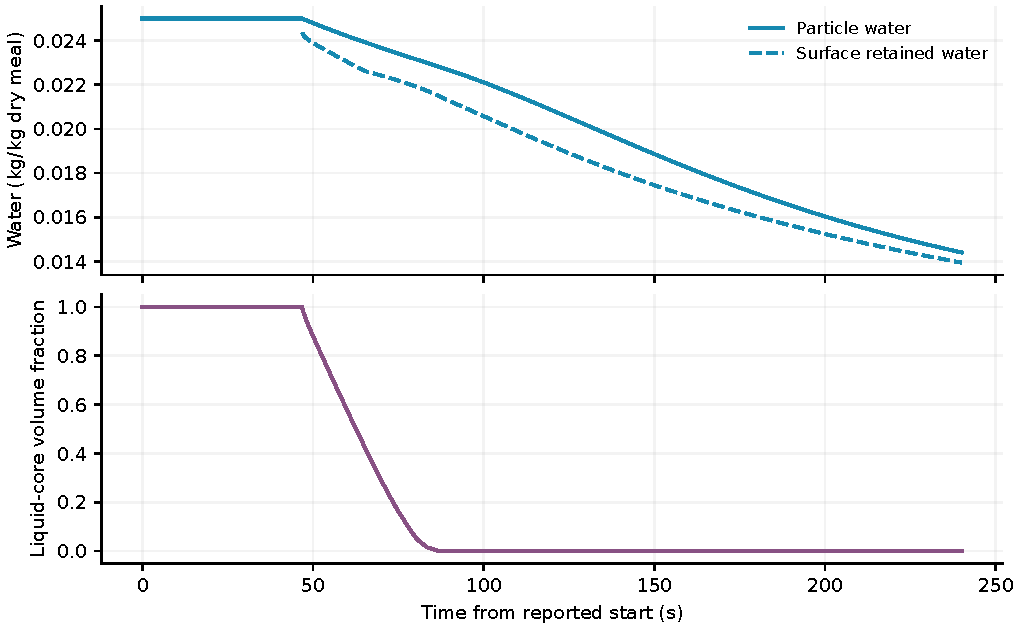
\includegraphics[width=0.9\textwidth]{figures/fig_faner_supporting_states.pdf}
\caption{Faner particle: retained water and liquid-hexane core volume fraction.}
\label{fig:fanersupport}
\end{figure}

\section{Process interpretation, sensitivity and limits}
\label{sup:missingfull}\label{sup:extrapolationflags}\label{sup:regime}\label{sup:regimegrid}\label{sup:desolventizerfloor}\label{sup:envelopescoring}\label{sup:identifying}
This section relates the particle results to the DT and states each comparison's scope. A process model needs both a particle source or sink and the gas and meal histories on a tray; this paper supplies only the first. Depletion of external free hexane allows the dry shell to form, but a tray model must still account for particles arriving at different loadings and sizes, steam condensation, finite residence, gas composition, mixing, jacket heat and vapour escape. A film coefficient deduced on a thin holder cannot be applied unchanged to an industrial bed, and the sample's local heat path and probe position were not measured.

Within its modeled range, at the constant gas state of each separate march,
the moving-front formulation is heat-fed: the binary pore mobility separates
water from n-hexane but adds no independent resistance to their total
escaping flux. For the \emph{separate Fickian dry-shell comparison}, the
ratio of conductive heat supply, expressed as an evaporation flux, to
diffusive solvent supply is
\begin{equation}
\Lambda=\frac{k_{\mathrm{dry}}(T_{\mathrm g}-T_{\mathrm{int}})
                  /\Delta h_{\mathrm{vap}}(T_{\mathrm{int}})}
                {D_{\mathrm{eff}}[c_{\mathrm{sat}}(T_{\mathrm g})-c_{\mathrm s}]},
\label{eq:sub:bottleneck}
\end{equation}
where $c_{\mathrm{sat}}$ and $c_{\mathrm s}$ are the n-hexane mass
concentrations at saturation and at the particle surface, respectively.
On the declared gas-state grid, $\Lambda$ ranges from $7.80\times10^3$ to
$6.29\times10^4$ over states with a receding front. A value above unity
means that this Fickian comparison is limited by its assumed solvent
transport. The ratio is not the moving-front model's vapour resistance; the
grid is not a set of integrated drying trajectories and does not identify
the resistance acting in a measured tray of steam-wet meal.

Table~\ref{tab:sub:scope} summarizes what each comparison establishes and
the measurements needed to distinguish the remaining mechanisms (DTDC:
desolventizer-toaster-dryer-cooler).

\begin{table}[htbp]\centering\footnotesize
\caption{Scope of the benchmark evidence.}\label{tab:sub:scope}
\begin{tabular}{@{}>{\raggedright\arraybackslash}p{0.28\textwidth}>{\raggedright\arraybackslash}p{0.34\textwidth}>{\raggedright\arraybackslash}p{0.30\textwidth}@{}}\toprule
Claim & What is actually tested & Missing discriminator\\\midrule
Heat-fed surface period & Four measured duties under a declared mass basis and an independent packed-bed correlation & Source-specific exposed area and per-run state\\
Slow Fickian shell & Two 2008 measured trajectories with one surface-read coefficient from uptake & Thesis particle shape, local-coefficient convergence, high-temperature transport\\
2019 water-bearing particle & A four-cell radial particle with film from the constant rate; falling-rate loading is faster than the measured charge & Measured mass-weighted size histogram, wetness near the probe, its depth and gas flow through the holder\\
Binary water--hexane storage/transport & Conservation and limiting-case numerical identities; no measured two-component drying trajectory & Water-isotherm and co-sorption data; coupled moisture and solvent profiles\\
Industrial DT/DTDC & One radial particle on a declared bath; solvent, moisture and temperature lie within the published outlet ranges; Coletto et al.'s column integration is not the boundary, because its flashing zone uses eq.~A.17 and its toaster particle step has no water balance & Independent tray gas, steam, wall, residence and discharge observations\\
\bottomrule\end{tabular}\end{table}

With pressure and source-water-isotherm alternatives propagated, the sorption-elevated boiling condition $a_{\mathrm w}(\Xw)P_{\mathrm{sat}}^{\mathrm w}(T^*)=P$ of the main text gives $100.5$--$107.6$ degrees Celsius, a range spanning a published band of industrial discharge temperatures. The single point at the moisture of the temperature source itself lies 2.05 kelvin above that band. This is a cross-source check of equilibrium \emph{at supplied moisture}, not a drying trajectory of wet meal. At declared last-tray hexane mole fractions $0.003$--$0.03$ and temperatures 100--110 degrees Celsius, a dry-particle equilibrium calculation gives $4.5$--$66.0$ ppm without and $8.1$--$112.4$ ppm with a residual-oil solution arm (Sec.~\ref{sup:evidence:outlet}); only the richest and coolest oil-arm corner reaches the published residual-hexane class. This floor is not a simulated tray-discharge concentration. The total-meal GAB isotherm already includes reference oil, so the overlap with the oil arm is an explicit uncertainty, not an independently established extra inventory.

Four groups of extrapolations or omissions limit the process reading. The GAB hexane isotherm is evaluated above its fitted temperatures or below some measured activities. The modified Luikov water isotherm has no soybean-meal data near desolventizer temperature, and its binary co-sorption evidence is narrow. The cross-virial gas interaction is an interval, not a measured term for every operating state. The declared binary pore diffusivity and reference retained-water mobility are not identified from coupled drying data on this soybean meal. Shrinkage, a Darcy or Knudsen resistance on the total vapour flux, a distributed instead of sharp phase change, and re-wetting of a receded core are not identified mechanisms here. Three groups of transport and surface coefficients have positive intervals without source-backed endpoints. No adjustment of numerical residual tolerances can make up for these missing material data.

The experiments that would settle the remaining physical questions are specific: (i) a pure-hexane series on one meal at two controlled particle sizes, with temperature logged through the crossing; (ii) a mass-weighted size histogram, effective exposed area and wetness map around each thin-layer thermocouple; (iii) a high-temperature series of effective solvent transport on the same meal, read through the sorption isotherm; (iv) moisture profiles and a water isotherm at process temperature; and (v) transient solvent \emph{and} water measurements in a steam-exposed particle or thin layer with a known gas supply. At equipment scale, a particle-plus-tray DT calculation needs an independent published or plant record of feed, vapour, steam, wall duty, temperature and discharge, followed by the dryer-cooler and the whole-tower residence distribution. The present comparisons are a foundation for those tests, not a substitute for them.

\section{Comparison inputs, uncertainties and source limitations in detail}
\label{sup:detail:inputs}\label{sup:detail:numerics}\label{sup:detail:ensemble}
This section gives the inputs of each measured-curve comparison and the source statements behind them. The comparisons carry three kinds of uncertainty, which are not combined into one error bar: the reading half-width of a point digitized from a published trace; a source statement (mass basis, particle shape, probe depth, gas flow) that admits more than one reading, each an alternative model input, not a sample from a distribution; and the covariance or prediction interval of a coefficient fitted to independent data, which does not cover a temperature extrapolation or an unmeasured geometry. The main text states the strongest condition beside each headline result.

\subsection{Which source statements set a calculation}
For the 2008 thesis, the nominal sample mass is read as the wet charge, because the printed flux definition then reproduces the plotted constant-rate slope; reading it as dry meal predicts much less duty and a later transition, and the two readings cannot be averaged. Within a source, a tabulated quantity takes precedence over a position digitized from a graph, and a later peer-reviewed statement of a condition over an earlier thesis sentence. On version two of the digitization, the thesis sunflower window holds fourteen points from the measured crossing on. The earlier $9.1$-percent residual on the 2019 sunflower sphere belongs to version one ($14$ of $15$ in band); rescored on version two it is $11.6$ percent ($13$ of $14$), a change of the scored reading, not of the equations. For the 2019 run, the particle sizes and sphericity come from the article; the current experiment declares one representative radius because no mass histogram of the charge is printed. The film exposure multiplier comes from the constant-rate slope; the gas flow through the holder, the wetness near the thermocouple and its depth remain unmeasured (Sec.~\ref{sup:journalmarch}).

\subsection{External heat coefficient and finite sample geometry}
\label{sup:detail:geometry}
\paragraph{Film exposure multiplier: source data and calculation.}
\label{sup:fanermultiplier}
The multiplier was inferred from the constant-rate evaporation duty, including the Ackermann correction. For a
sphere with a wet surface,
$m''\Delta h_{\mathrm{vap}}=h_Q\Phi(\beta)(T_g-T_b)$ and
$r_c=3m''/(\rho_{\mathrm{dm}}\Rp)$, where $r_c$ is the decline of
hexane loading per unit dry mass and $\beta=m''c_{p,\mathrm v}/h_Q$.
The original construction matched mass-weighted particle rates to a
least-squares source slope of $7.26\times10^{-3}$ kg/(kg dry s), using
the four soybean solvent-loading readings in Fig.~2 of
\citet{faner2019kinetics}, above loading 0.2388. The digitized pairs
$(t_j\text{ [s]},X_j\text{ [kg/kg dry]})$ are
\[
\begin{aligned}
 &(0.000,\;0.492364),\quad(9.884,\;0.420900),\\
 &(20.077,\;0.337384),\quad(29.961,\;0.278064).
\end{aligned}
\]
These values keep the digitization precision for reconstruction; it does
not represent experimental accuracy.
With bars denoting the four-point arithmetic means, the slope is
\[
r_c=-\frac{\sum_j(t_j-\bar t)(X_j-\bar X)}
                  {\sum_j(t_j-\bar t)^2}
    =7.260603\times10^{-3}\ \mathrm{kg/(kg\ dry\ s)}.
\]
The construction used a truncated lognormal number distribution of sizes,
consistent with the reported mean diameter and size fractions and converted
to mass weights, with reference radius 0.666 mm and initial loading 0.4924.
For each size class $i$, the Ackermann balance gives
\[
r_i(f)=\frac{3f h^0_{Q,i}}{\rho_{\mathrm{dm}}R_i c_{p,\mathrm v}}
 \ln\!\left(1+\frac{c_{p,\mathrm v}(T_g-T_b)}
 {\Delta h_{\mathrm{vap}}}\right),
\]
where $h^0_{Q,i}$ is the unscaled correlation coefficient.
The earlier ensemble uses 400 mass-weighted classes. It chooses the
single factor $f$ so that the least-squares decline of its mean loading,
$\bar X(t;f)=\sum_i w_iX_i(t;f)$, at the same four times equals $r_c$.
The smallest classes enter the falling-rate period inside that window;
matching only the ensemble's initial rate would give 0.14508.
The four-time rule gives $f=0.1457854364$; the present 0.885-mm particle
uses it unchanged, with initial loading 0.475.
The multiplier is therefore a boundary calibration carried over from an
earlier geometry, not an independently measured transport property or
exposed surface fraction. The later falling-rate and temperature readings
were not used to identify it.
The digitized data, distribution inputs, slope calculation and exact
carried-over value are recorded in the reproducibility file
\texttt{faner\_film\_boundary\_derivation\_2026-10-08.json}.

The unscaled gas-film heat and mass coefficients use an industrial
reference superficial velocity of 0.230 m/s, obtained from a 3.9 kg/s gas
flow, a 6-m tower diameter, a gas density of 0.60 kg/m$^3$ and a bed voidage
of 0.40 \citep{coletto2022modeling}. At the present reference radius, the
heat coefficient is 104 W/(m$^2$ K) and the mass coefficient 0.0672 m/s;
scaling gives 15.1 W/(m$^2$ K) and 0.00980 m/s. Both coefficients
are scaled, while the geometric area remains $4\pi\Rp^2$.
The heat-duty inference does not determine mass transfer separately,
so applying the same factor to both is a declared boundary assumption.
Faner's charge of about 30 g in a 0.011-m$^2$ holder forms a layer
about three to five particle diameters deep \citep{faner2019kinetics}.
The industrial reference coefficients cannot be assumed to describe that
holder without a separate assessment of its gas flow and sample contact.

An unscaled calculation, with multiplier one and otherwise the same
four-cell particle, initial moisture, oil fraction, transport coefficients
and prescribed vapour, depletes external free hexane at 6.8 s and crosses
0.20 kg/kg dry at 6.8 s, rather than 46.8 s and 46.6 s, respectively.
Its heat and mass coefficients are 6.86 times larger. The calculation
enters regime B and continues to 6.88 s with the same component
and energy checks; the bounded continuation then reaches its computing-time
limit. This result shows the early boundary sensitivity; it is not a
complete falling-rate history or a prediction of the later temperature.

Separately, at the 2008 rig's own state, Whitaker's packed-bed correlation
predicts $0.82$--$1.06$ of the constant-rate duties on the wet-charge
basis (Sec.~\ref{sup:filmmatch}). Two inferred coefficients lie $3.7$ and
\SI{4.2}{\percent} below it, so the bracketing criterion over three
correlations, declared before the comparison, is narrowly missed; the film
is reported as a duty comparison with the departure stated. A tray
comparison needs its own gas composition, voidage, interfacial area and
condensation balance; the holder's coefficient cannot simply be copied.

\subsection{The declared spheres and the effective diffusivity law}
This subsection details the declared spheres and diffusivity law of Sec.~\ref{sup:surfaceloading}. The convention $R_d=\psi d_{\mathrm{eq}}/2$ gives the sphere the particle's volume-to-surface ratio. It was adopted after the effective-radius sensitivity had been inspected and is an assumption for the 2008 samples, whose shape was not measured; the 2019 sphericity $0.74$ comes from later samples. At constant diffusivity the spherical diffusion time scales with $\Rp^2/\Deff$, so a drying curve alone cannot separate radius from diffusivity. The volume-to-surface equivalence is an early-time construction, while the scored window reaches a Fourier number near $0.3$. The law's temperature term is weakly resolved (the 95-percent half-width of the activation energy exceeds its central value), and its prediction factor is a spread within the regression domain, not a statement about the \SI{41}{\kelvin} transfer above it. Reading the coefficient at a weighted mean concentration instead of at the surface would raise it five- to seventy-five-fold and dry far too fast; reading it in each interior cell gave no mesh-refined solution.

Table~\ref{tab:detail:geometry} compares these sphere conventions with
the same coefficient law. Errors are RMS fractions of the measured loading
drop; parentheses count points within the reading band, out of fourteen sunflower and fifteen soybean observations.

\begin{table}[htbp]\centering\footnotesize
\caption{Particle geometry sensitivity in the 2008 falling-rate comparisons.}
\label{tab:detail:geometry}
\begin{tabular}{@{}>{\raggedright\arraybackslash}p{0.49\textwidth}cc@{}}\toprule
Sphere convention & Sunflower & Soybean\\\midrule
Thesis volume-equivalent diameter & $0.379$ ($1$) & $0.310$ ($1$)\\
2019 soybean volume-equivalent diameter, both traces & $0.317$ ($1$) & $0.303$ ($1$)\\
$\psi$ times thesis sample diameter, declared & $0.172$ ($9$) & $0.156$ ($8$)\\
$\psi$ times 2019 soybean diameter, both traces & $0.099$ ($14$) & $0.147$ ($9$)\\
$\psi$ times 2019 sunflower diameter, sunflower only & $0.116$ ($13$) & --\\
\bottomrule\end{tabular}\end{table}

Table~\ref{tab:detail:dryladder} tests mesh and time-step sensitivity
on each thesis sample's declared sphere. It reports the RMS error of the
surface-read Fickian calculation as a fraction of the scored loading drop.

\begin{table}[htbp]\centering\footnotesize
\caption{Space and time refinement of the 2008 Fickian comparisons.}
\label{tab:detail:dryladder}\label{tab:evidence:dryladder}
\begin{tabular}{@{}lccc@{}}\toprule
Trace & 60 cells, nominal step & 120 cells, quarter step & 240 cells, quarter step\\\midrule
Sunflower, $\Rp=0.7215$ mm & $0.1721$ & $0.1678$ & $0.1676$\\
Soybean, $\Rp=0.6660$ mm & $0.1562$ & $0.1525$ & $0.1524$\\
\bottomrule\end{tabular}\end{table}

Across the law's prediction band, the residual on the declared sunflower sphere runs from $5.4$ to $52.6$ percent and on soybean from $7.7$ to $42.2$ percent; the best match lies inside the band, so points inside a broad band do not identify a mechanism. The central marches dry more slowly than both traces. Even so, a storage-consistent path with no coefficient fitted to the falling-rate points comes considerably closer than the same law on the volume-equivalent spheres. The uncertainty is dominated by particle shape and source conditions, not by truncation error in the surface-read form.

\section{Reproducing the comparisons: inputs, scores and stopping conditions}
\label{sup:protocol}\label{sup:protocol:availability}
\subsection{What is compared, and on which time origin}
Every comparison in the main text names its observation and actual time
origin; this section gives them, with the scores. The source
records solvent loading per kilogram of dry meal and one holder thermocouple.
The 2008 scalar Fickian shell starts at a measured loading crossing and is
scored separately. The 2019 comparison uses a radial water-bearing particle
with a declared initial state and the constant-rate film exposure
multiplier. No time shift is applied to reduce its falling-rate
discrepancy. The measured and calculated $X_{\mathrm h}=0.20$ crossings are
45.9 s and \FanerCrossTwenty{} s. Their respective intervals to 0.10 kg/kg
are 25.4 s and \FanerFallingInterval{} s.
Crossings are interpolated linearly between successive calculated states;
lines in a figure are not additional solved states. The calculated
temperature is a volume-mean particle temperature, not a local holder
thermocouple reading. Since the heat supply was identified on this run, the onset time is not
an independent prediction of the film. Section~\ref{sup:journalmarch}
gives the initial-water and preheat uncertainty, mesh and time-step
sensitivity, and the component, energy and whole-history checks.

\subsection{Scores and uncertainty conventions}
The band around a digitized point is the reading half-width of this digitization, not an experimental standard deviation; a point \emph{in band} lies within that resolution. The RMS drying score is the root mean square of model minus measured loading over the scored window, divided by the measured loading drop over that window. Changing a class distribution, coefficient or window defines a new calculation, not a new reading of the same score. The regression of converted uptake coefficients states 95-percent half-widths on its exponents and a residual standard deviation in log coefficient; neither covers the thesis samples' geometry or the \SI{41}{\kelvin} transfer. Faner's image-analysis counts give neither a mass-weighted histogram nor the thermocouple's local wetness, and the digitization half-widths represent neither uncertainty.

Table~\ref{tab:protocol:scoring} summarizes the observations and metrics
of the separate comparisons and what each does not establish. Each score is
thus tied to one observation, time origin and scored window.

\begin{table}[htbp]\centering\footnotesize
\caption{Observations, comparison metrics and interpretation limits.}
\label{tab:protocol:scoring}
\begin{tabular}{@{}>{\raggedright\arraybackslash}p{0.23\textwidth}>{\raggedright\arraybackslash}p{0.34\textwidth}>{\raggedright\arraybackslash}p{0.35\textwidth}@{}}\toprule
Observable & Input and metric & Not established\\\midrule
Constant-rate duty & Rig gas and holder state, Whitaker film, measured slope; computed over observed duty & An intraparticle drying law, or an area valid on industrial trays\\
2008 falling-rate loading & Surface-read, storage-corrected Fickian shell; RMS over the window drop & A moving-front march, or the thesis samples' shape\\
2019 thermocouple & Four-cell representative-particle mean temperature compared diagnostically with one local holder probe; departure time and RMS & Particle mean is not local probe temperature; wetness and depth near the probe\\
2019 loading tail & One declared sphere and constant-rate film; time from crossing to $0.10$ and window RMS & Charge-specific mass-weighted size histogram; a fit to later loading\\
Uptake at \SI{50}{\celsius} & Coefficient conversion identified on the same measured curves & A held-out transport prediction at process temperature\\
Desolventizer march & Declared bed history and deck duty, published envelope; station values & A tray trajectory or a measured discharge residual\\
\bottomrule\end{tabular}\end{table}

\section{Property domains and process boundaries}
\label{sup:propertyledger}
The particle formulation's property evidence is uneven; Table~\ref{tab:protocol:domains} states what each closure rests on and where it is open. The formulation carries hexane as mobile liquid, sorbate and pore gas, and water as retained and pore-gas inventories. A pure n-hexane inlet lies outside the measured water-activity range of the default binary interface formulation at the relevant temperature. The current pure bulk vapour is evaluated separately from the binary pore and surface state, while positive retained water remains active after the shell forms. The analytic low-water continuation is stated explicitly (Sec.~\ref{sup:journalmarch}).

\begin{table}[htbp]\centering\footnotesize
\caption{Property evidence and unresolved model assumptions.}
\label{tab:protocol:domains}
\begin{tabular}{@{}>{\raggedright\arraybackslash}p{0.25\textwidth}>{\raggedright\arraybackslash}p{0.35\textwidth}>{\raggedright\arraybackslash}p{0.32\textwidth}@{}}\toprule
Closure or path & Source-supported information & Outside or unresolved\\\midrule
Hexane retention on reference meal & GAB fit on soybean meal containing residual oil; activity, loading and fitted temperature span from \citet{cardarelli1996hexane} & Process-temperature extension; an oil arm is not an independent inventory\\
Water retention & Modified Luikov law and low-temperature meal measurements; capacity and lower anchor explicit & High-temperature soybean sorption and mixed water/hexane occupancy unmeasured\\
Binary pore gas & Thermodynamic-force exchange plus continuity-derived total flux & Binary mobility and bulk-flow resistance unmeasured for this meal\\
Retained-matrix water & Separate water mobility and an exposed-surface path & Neither identified on this meal\\
Pure-hexane bath particle & Water-bearing radial particle, constant gas, film exposure multiplier, conservative core disappearance and stationary radial tail & Initial moisture/preheat, local bed geometry, mass-weighted sizes and robustness of shell formation at high moisture\\
2008 effective solvent shell & Apparent uptake coefficients converted for sorption storage, read once per step at the surface & High-temperature extrapolation, sample shape, local-law convergence\\
Oil-arm equilibrium floor & Four external oil/hexane determinations & Overlap with the total-meal fit unmeasured\\
\bottomrule\end{tabular}\end{table}

\section{Gas-composition and outlet-equilibrium calculation}
\label{sup:evidence:outlet}\label{sup:evidence:checks}\label{sup:evidence:outstanding}
This section gives the equilibrium calculation behind the residual-hexane floor quoted in the main text. The pressure-feasible solvent activity used for the outlet check is $a_{\mathrm{h}}^{*}=\min(1,\yh P/P_{\mathrm{sat}}^{\mathrm{h}}(T))$. An equilibrium at a specified $y_h$ and temperature gives an \emph{equilibrium loading}, not the time to reach it. Table~\ref{tab:evidence:floor} separates GAB-retained solvent from the total dry-shell inventory, which also holds pore gas; its grid is a literature-based range of last-tray states, not a plant sensor trace. The last-tray total of $4.5$--$66.0$ ppm without the oil-solution arm refers to $y_h=0.003$--$0.03$ and 100--\SI{110}{\celsius}. With the oil-dissolution sensitivity it becomes $8.1$--$112.4$ ppm; this band must not be formed by adding the arm to a total-meal isotherm as if their overlap had been measured. In the experiments' pure-hexane gas the floor is many times higher. The DT march of Sec.~\ref{sup:dtmarch} reads this floor at its declared exit gas, $y_h=0.01$, below the dry-shell tail.

Table~\ref{tab:evidence:floor} uses a pressure of \SI{101.3}{\kilo\pascal}.
The $y_h=1$ row represents the experimental pure-hexane gas, not
a desolventizer exit. The oil-solution sensitivity (Sec.~\ref{sup:missingfull})
is not included in the table totals.

\begin{table}[htbp]\centering\footnotesize
\caption{Equilibrium hexane inventories at atmospheric pressure (ppm dry meal).}
\label{tab:evidence:floor}
\begin{tabular}{@{}r rrrr@{}}\toprule
 & \multicolumn{2}{c}{\SI{100}{\celsius}} & \multicolumn{2}{c}{\SI{110}{\celsius}}\\
\cmidrule(lr){2-3}\cmidrule(lr){4-5}
$y_h$ & Sorbed & Total & Sorbed & Total\\\midrule
$0.003$ & $5.55$ & $6.58$ & $3.51$ & $4.51$\\
$0.01$ & $18.52$ & $21.94$ & $11.71$ & $15.04$\\
$0.03$ & $55.76$ & $66.02$ & $35.24$ & $45.24$\\
$0.10$ & $188.23$ & $222.45$ & $118.90$ & $152.22$\\
$1.0$ & $2312.41$ & $2654.60$ & $1416.61$ & $1749.88$\\
\bottomrule\end{tabular}\end{table}

Two numerical checks mark the limits of the coupled form rather than validate it. In the ideal-binary reduction the scalar Fick identity holds to $6.34\times10^{-16}$, while at finite pressure the low-water coefficient comparison leaves a \SI{3.799}{\percent} discrepancy that no calibration sets to zero. The default coupled interface formulation at \SI{409.15}{\kelvin} admits a pore hexane fraction of at most $0.857$; this restriction does not define the supplied external bath. The Faner experiment with a water-bearing particle treats the pure bulk gas separately from its binary state in the pores and at the surface; the earlier property-table checks are separate from this march. The experiments that would settle what the comparisons leave open are listed at the end of Sec.~\ref{sup:missingfull}.

\section{The prescribed DT bath and particle history}
\label{sup:dtmarch}
This section documents the main-text DT experiment. It prescribes the gas bath instead of
solving tray vapour and energy balances. It uses the same particle
conservation laws, positive-water retention branch and gas and matrix
transport coefficients as the Faner experiment. The external water film
stores water and energy separately, and liquid-water imbibition transfers
water into the dry shell while the film is present. The surface closure adds
no water-film resistance to hexane escape. No front temperature or
particle-temperature history is imposed.

\paragraph{Inputs.}
The prescribed residence is 1766.535501 s and the effective spherical
radius is 1.5 mm. This is a selected coarse-particle case; the main text
states its origin and distinguishes it from a measured DT mean radius.
Feed temperature is 322.15 K, hexane loading 0.387786 kg/kg dry meal,
retained water 0.123664122 kg/kg dry meal and oil fraction 0.013740458.
The pre-desolventizing (PD) bath is 345.15 K, with hexane mole fraction
0.6644429974, exposure fraction 0.004081 and indirect duty 85 W/kg dry
until 490.202242 s. The steam-rich bath then ends at 378.15 K;
its gas states and timings are recorded in
\texttt{destiny\_v3\_exit105.json}. These inputs define a scenario,
not a measured plant bath or a new countercurrent-column calculation.

\paragraph{Shared particle closure.}
Both experiments use binary pore diffusivity $6\times10^{-10}$ m$^2$/s,
reference retained-water mobility $8.47\times10^{-7}$ mol/(m s),
conductivity 0.24 W/(m K), equation-of-state fugacities, retained-component
state functions and component-consistent energy. The positive-water
Luikov extension is stated in Sec.~\ref{sup:journalmarch}. Initial water, oil
and radius differ between the experiments; the constitutive laws do not.
Liquid-water imbibition uses the liquid contact conductance $K_\ell=0.32$ mol/(m$^2$ s) and a total-to-reference
shell mobility factor of 1000, as derived in Sec.~\ref{sup:finitecontact}.
The pathway is inactive in the Faner experiment, which has no water
film.
Regime A uses a uniform-temperature particle coupled to a separate
surface; regimes B and C use two radial cells. These coarse
representations are stated numerical limitations.

\paragraph{Events and exit.}
External free hexane is depleted at 492.257073 s, and the first dry-shell
interval ends at 492.267073 s. Regime B resolves the front's grid-face
arrival and departure before core extinction at 503.560810 s. The external water film stays positive throughout regime B.
Regime C advances the stationary radial particle and water film together,
resolves film depletion at 624.548745 s and continues to the prescribed
exit at 1766.535501 s. Final core volume and external water film are zero.
Particle water is 0.222554024 kg/kg dry, hexane is 0.000135230559 kg/kg dry
and volume-mean temperature is 378.125370 K.

Wet-basis moisture is $100X_{\mathrm w}/(1+X_{\mathrm w}+X_{\mathrm h})$,
giving 18.2020\%. Residual hexane is 135.231 mg/kg dry, or 110.601 ppm
on a wet basis with the same denominator. This conversion excludes the water
stored in the external film. Figure~\ref*{M-fig:dtmarch} of the main text
places the published outlet ranges at 30 min for visual reference; the
computed clock and its earlier end point are not shifted. The published
ranges are process context, not measurements of this particle or bath.

\paragraph{Conservation and numerical scope.}
An independent reconstruction covers every accepted step from
dry-shell formation to exit, evaluating water, hexane and energy in the
particle and external water film. The maximum normalized defects are
$4.24\times10^{-11}$, $8.61\times10^{-13}$ and $6.16\times10^{-12}$,
respectively.
The preceding feed history keeps its separate check. Regime-C step
halving is reported in Sec.~\ref{sup:finitecontact}. Whole-history mesh
and time-step convergence has not been demonstrated, nor has the regime-B
branch with a depleted film; the actual regime-B trajectory keeps a positive
film and therefore does not exercise that branch.

Each segment records its source-file hashes and starting checkpoint. Auxiliary code was developed between runs, so these records do
not form one fixed, executable replay. The reproduction package must
preserve the actual sources, inputs, histories and legally distributable
measured data. Conservation and numerical checks support the reported
discrete experiment; they do not identify the unmeasured material
coefficients or validate an industrial DT.

\section{Liquid-water imbibition: coefficient basis and numerical evidence}
\label{sup:finitecontact}
This section derives the water-transport coefficients of the particle and
gives the numerical evidence for the DT calculation with liquid-water
imbibition. Imbibition is part of the particle formulation and
is active only while the external water film contacts the dry shell. It is
inactive in the Faner experiment, which keeps the reference pore-gas
and retained-water fluxes. Its external series resistance, film-stock limit and energy transport
are given in the main text.
It introduces no extra water storage or retention capacity.

\paragraph{Material interpretation.}
Liquid-water imbibition into soy protein isolates combines adsorption,
capillarity and loosely held interstitial water, and its capacity exceeds
equilibrium vapour sorption several-fold \citep{jovanovich2003wateruptake}.
Assigning the incoming liquid to one retained-water inventory is an
effective closure, not a measurement of its microscopic phase partition. Displacement of hexane by water, swelling, liquid
pressure and blocking of hexane by water are outside this closure.

\paragraph{Reference transport coefficients.}
The reference binary pore value $D_b=6.0\times10^{-10}$ m$^2$/s is an
engineering sensitivity point, 1.5 times the scalar diffusivity used by
\citet{cardarelli2002modeling}. The reference retained-water mobility is derived
from the linearized coupled balances at $T=385.65$ K, $P=130$ kPa and
$y_{\mathrm h}=0.80$, with the reference retention properties.
Eliminating the total molar flux gives the local apparent response
\[
D_{\mathrm{app}}=D_{\mathrm{app,pore}}+g_{\mathrm{ret}}\mathcal L_{\mathrm{w,ret}},
\]
where $D_{\mathrm{app,pore}}=4.54\times10^{-12}$ m$^2$/s and
$g_{\mathrm{ret}}=7.26\times10^{-4}$ m$^3$/mol are obtained from the
same storage and chemical-potential derivatives. Setting the combined
response to $6.2\times10^{-10}$ m$^2$/s gives the reference retained-water
mobility $8.47\times10^{-7}$ mol/(m s). The target value is the maximum apparent
moisture diffusivity reported by \citet{touffet2026moisture} for
pelleted feed at \SI{60}{\celsius}; transferring it to this reference
state is an engineering assumption. On the isothermal, uncapped Luikov
branch, the diffusivity of the retained-water path is
\[
D_{\mathrm{ret}}=
\frac{M_{\mathrm w}\mathcal L A_1}{\rho_{\mathrm{dm}}A_2W^2},
\]
which for the reference mobility is $3.8\times10^{-10}$ m$^2$/s at
$W=0.05$ and $2.4\times10^{-11}$ m$^2$/s at $W=0.20$. That span covers
the two available measurements on oilseed meal: vapour-sorption diffusivities of
sunflower meal, $10^{-12}$ to $1.15\times10^{-10}$ m$^2$/s at
50--\SI{95}{\celsius} \citep{cardarelli1998thesis}, and the soaking
diffusivity of defatted soybean meal, $1.14$ to $2.07\times10^{-11}$
m$^2$/s at 20--\SI{60}{\celsius} \citep{mukherjee2019soaking}. The
reference retained-water mobility is therefore consistent with oilseed meal, although
its value was taken from the pellet study.

\paragraph{The liquid-water mobility factor.}
The liquid-water mobility is $\mathcal L_\ell=999\,\mathcal
L_{\mathrm{w,ret}}=8.47\times10^{-4}$ mol/(m s), so the total shell
mobility is the reference value times a mobility factor of 1000. The
number is the span of the liquid transport
coefficient of porous hygroscopic solids between the dry state and
free water saturation, which \citet{kunzel1995simultaneous} measured on
bricks, sandstones and concretes and expressed as
$1000^{\,w/w_f-1}$ with $w_f$ the free saturation (his eq.~24). In the
sorption region of the same materials the liquid contribution is only
one to two times the vapour transport, so a constant factor is the
water-filled-pore limit of that law. We apply it because the pathway is
active only in the dry shell while the external water film is filling
its pores. Starting from the reference retained-water mobility, $D_{\mathrm{ret}}$ at $W=0.20$ is
$2.4\times10^{-8}$ m$^2$/s on the enhanced pathway.

The mobility factor and the liquid contact conductance act in series, with
the interior
term $d/\mathcal L_\ell$ and the surface term $1/K_\ell$, so a single
uptake time fixes only their sum. Table~\ref{tab:finitecontact:factor}
gives the interior share of the series resistance at the DT radius with
$d=\Rp/5$, the lumped-sphere equivalent, for $K_\ell=0.32$ mol/(m$^2$ s).
Above a factor of about 300 the surface controls the uptake and the
result no longer depends on the factor. Below 100 the interior would
double the resistance, and the conductance derived below would have to
rise to reproduce the same measurement. Completed DT marches at factors
100, 1000 and 10\,000 with the same $K_\ell$
(Table~\ref{tab:finitecontact:factormarch}) confirm this. The tenfold
reduction to 100 lowers the outlet moisture by 0.58 percentage points
and raises hexane by 22.8 mg/kg dry; the tenfold increase to
10\,000 moves them by only $+0.07$ points and $-2.7$ mg/kg dry. The
outlet is on its plateau at 1000.

\begin{table}[htbp]\centering\small
\caption{Interior share of the series resistance to liquid entry at the
DT radius, $K_\ell=0.32$ mol/(m$^2$ s), $d=\Rp/5$.}
\label{tab:finitecontact:factor}
\begin{tabular}{@{}rrr@{}}\toprule
Mobility factor & Interior share & Uptake slowdown vs.\ contact alone\\\midrule
30 & 0.79 & 4.8\\
100 & 0.53 & 2.1\\
300 & 0.27 & 1.4\\
1000 & 0.10 & 1.1\\
3000 & 0.04 & 1.04\\
\bottomrule\end{tabular}\end{table}

\begin{table}[htbp]\centering\small
\caption{DT outlet against the liquid-water mobility factor at
$K_\ell=0.32$ mol/(m$^2$ s); every other input as in
Table~\ref{tab:finitecontact:sensitivity}. The last column gives the
maximum normalized water, hexane and energy defects of the independent
reconstruction from dry-shell formation to exit (acceptance $10^{-10}$).}
\label{tab:finitecontact:factormarch}
\begin{tabular}{@{}rrrrrrl@{}}\toprule
Factor & Moisture, \% wet & Hexane, mg/kg dry & Hexane, ppm wet & Mean $T$, $^\circ$C & Film consumed, s & W / H / U defects\\\midrule
100 & 17.62 & 158.0 & 130.1 & 105.01 & 702.5 & $7.1\times10^{-12}$ / $2.1\times10^{-12}$ / $2.7\times10^{-12}$\\
1000 (adopted) & 18.20 & 135.2 & 110.6 & 104.98 & 624.5 & $4.2\times10^{-11}$ / $8.6\times10^{-13}$ / $6.2\times10^{-12}$\\
10\,000 & 18.27 & 132.5 & 108.3 & 104.97 & 614.0 & $2.6\times10^{-11}$ / $2.8\times10^{-12}$ / $4.4\times10^{-12}$\\
\bottomrule\end{tabular}\end{table}

\paragraph{Construction of the contact conductance.}
\label{sup:contactscale}
The liquid contact conductance represents the resistance to liquid entry
between the external water film and the connected particle matrix. It keeps
the surface conductance finite when the shell forms, where the main-text law
gives $G_\ell\to K_\ell$ as $d\to0$. Its value is derived from the only kinetic
measurement of solvent-extracted soybean meal in liquid water
\citep{hemmingsen2008water}: the coarse sieve fraction (above 0.5 mm,
mean 1.43 mm; 25 g fat per kg dry matter; initial water 11.8\%, that is
$W_0=0.134$ kg/kg dry) immersed at about \SI{80}{\celsius}: its
rehydration index is on its plateau at the first sample, 90 s, and
does not rise afterwards. The construction assumes a sphere of radius
$R=0.715$ mm, entry through the surface alone, the surface at the film's state
($W_{\mathrm{cap}}$) and the retention law of the main text. The water
balance $(\rho_{\mathrm{dm}}V/M_{\mathrm w})\dot W
=-A K_\ell[\psi(W)-\psi(W_{\mathrm{cap}})]$ with
$\psi(W)=(1-A_1/W)/A_2$ integrates in closed form to
\[
t=\frac{\rho_{\mathrm{dm}}R A_2}{3M_{\mathrm w}A_1K_\ell}\,
W_{\mathrm{cap}}\!\left[(W_0-W_1)+W_{\mathrm{cap}}
\ln\frac{W_{\mathrm{cap}}-W_0}{W_{\mathrm{cap}}-W_1}\right],
\]
and requiring $W_1=W_{\mathrm{cap}}-0.01$ kg/kg at $t=90$ s gives
$K_\ell=0.253$ mol/(m$^2$ s) at \SI{80}{\celsius}. Scaling the entry
rate with the inverse viscosity of water from 80 to \SI{100}{\celsius}
(a factor of 1.26) gives 0.318, adopted as 0.32. The end-point tolerance
is the largest single uncertainty of the construction: 0.02 or 0.005
kg/kg below capacity gives 0.21 or 0.43. Reading the measurement at
\SI{20}{\celsius} with the same construction and viscosity scaling
(a factor of 3.55) gives 0.90, so the adopted value is the lower,
less extrapolated, of the two readings.

The construction assumes that the sieve size is a sphere diameter, that
the interior had reached the retention capacity when the first sample was
drained, and that the entry rate scales with the liquid viscosity. The
measurement is on a drained filter cake and does not separate particle,
interstitial and surface water. The 90 s is therefore an upper bound on the
entry time, and the derived conductance is the slowest value consistent
with the measurement. It is a literature-derived value under these
declared assumptions, not a measurement on DT meal, and no DT outlet value
entered the calculation.

With the adopted liquid-water mobility, the resistance length
$\mathcal L_\ell/K_\ell$ is 2.65 mm, 1.76 times the DT radius. At
$d=\Rp$ the series conductance is $G_\ell=0.204$ mol/(m$^2$ s), and the
contact term's share of the series resistance is 0.64. The uniform-sphere linearization
$\tau_K=\rho_{\mathrm{dm}}\Rp A_2W^2/(3M_{\mathrm w}K_\ell A_1)$ gives
56 s at $W=0.20$, and the closed-form fill of a DT sphere limited by contact alone,
from the feed loading 0.124 to $W_{\mathrm{cap}}-0.01$, takes 153 s
(491 s in the earlier reference case 0.10). These are scale estimates;
radial gradients, pore-gas exchange, the changing surface state, the
film's water stock and the capacity all remain active in the calculation.

\paragraph{Sensitivity to the contact conductance.}
\label{sup:contactsensitivity}
Table~\ref{tab:finitecontact:sensitivity} lists completed DT marches at
four liquid contact conductances with every other input held constant,
the earlier reference case 0.10 among them. The outlet moisture is bounded by the condensate supply
and the retention capacity: the external water film is consumed before
the exit in every case, and a fourfold change in $K_\ell$ moves the outlet
moisture by 1.3 percentage points and the wet-basis hexane by 43 ppm.
The conductance sets how long the film persists, not how much water the
particle finally holds.

\begin{table}[htbp]\centering\small
\caption{DT outlet against the liquid contact conductance; mobility
factor 1000, two radial cells, regime-C maximum step 5 s, exit at
1766.5 s. Wet-basis values exclude the external film, which is zero at
the exit in every case.}
\label{tab:finitecontact:sensitivity}
\begin{tabular}{@{}rrrrrr@{}}\toprule
$K_\ell$, mol/(m$^2$ s) & Moisture, \% wet & Hexane, mg/kg dry & Hexane, ppm wet & Mean $T$, $^\circ$C & Film consumed, s\\\midrule
0.05 & 16.68 & 194.5 & 162.0 & 105.09 & 816.8\\
0.10 & 17.40 & 165.3 & 136.5 & 105.03 & 733.6\\
0.20 & 17.94 & 144.8 & 118.8 & 104.99 & 662.4\\
0.32 (adopted) & 18.20 & 135.2 & 110.6 & 104.98 & 624.5\\
\bottomrule\end{tabular}\end{table}

\paragraph{Events and refinement.}
The adopted DT calculation uses the feed history up to 492.257073 s,
effective radius 1.5 mm, two radial cells, the prescribed bath and the
existing retention capacity. The moving-front calculation begins with a
0.01-s shell-formation interval, advances regime B in 0.1-s intervals,
shortened where events require, and resolves grid-face arrival and departure
before core extinction at 503.560810 s. External water stays positive
throughout regime B, so the zero-film regime-B branch, which is not
implemented, is not exercised (Sec.~\ref{sup:dtmarch}).
Regime C advances the stationary particle and the film together to the
film's depletion at 624.548745 s and then to the exit.
Table~\ref{tab:finitecontact:refinement} gives the regime-C step
refinement, performed in the earlier reference case $K_\ell=0.10$ from the
same moving-front end point; the 5-s maximum step is used in every
reported march. The extra digits resolve the numerical sensitivity; the main
text uses rounded values.

\begin{table}[htbp]\centering\small
\caption{Regime-C timestep sensitivity of the DT particle with liquid-water
imbibition, $K_\ell=0.10$ mol/(m$^2$ s).}
\label{tab:finitecontact:refinement}
\begin{tabular}{@{}lrr@{}}\toprule
Quantity & Maximum step 10 s & Maximum step 5 s\\\midrule
Moisture, \% wet basis & 17.3813 & 17.4033\\
Hexane, ppm wet basis & 137.222 & 136.474\\
Mean temperature, $^\circ$C & 105.0329 & 105.0314\\
External-water depletion time, s & 735.395 & 733.575\\
\bottomrule\end{tabular}\end{table}

\paragraph{Independent balances.}
An independent reconstruction of the adopted march, from dry-shell
formation to exit, evaluates water (W), hexane (H) and energy (U) in the
particle and external water film at every accepted step. The maximum
normalized W/H/U defects are $4.24\times10^{-11}$, $8.61\times10^{-13}$ and $6.16\times10^{-12}$,
below the $10^{-10}$ acceptance limit; the regime-B segment alone gives
$1.05\times10^{-11}$, $8.61\times10^{-13}$ and $3.94\times10^{-12}$. The
unchanged feed history keeps its earlier check. Component partial
enthalpies count each energy transfer once. These checks show conservation in the
declared numerical experiment;
whole-history mesh and time-step convergence remains open
(Sec.~\ref{sup:dtmarch}), and conservation does not identify the material
coefficients.


\section{Reproduction inventory and accessibility}
\label{sup:deposit}
This section lists the released files and the planned release. At public
revision \texttt{f451d0e}, the preliminary package
distributes the analysis datasets and results as
\texttt{paper/analysis/datasets.zip},
\texttt{results\_2026-09-19.zip} and \texttt{results\_2026-10-01.zip}.
In the results ZIP files, member paths begin with the results-directory
name, not with \texttt{paper/analysis/}. The later results archive contains
earlier reduced continuations but not the current water-bearing particle
histories, and the public figure and supplement PDFs do not match this
submission. The updated release is being prepared to carry the particle
source code used to produce the results, the figure and table scripts, current run records, LaTeX sources and a SHA-256 manifest
tied to the source revision. Digitized readings and their reading
half-widths will be included only where redistribution is permitted;
otherwise the release will give an authorized access route. The authors'
code is under MIT terms, which do not cover the third-party publications or
their digitizations. Until the matching release and preservation archive
are available, the corresponding author can provide the current inputs and
records on reasonable request.

\clearpage
\section*{Nomenclature of the supplement}
\label{sec:si:nomenclature}
{\footnotesize
\setlength{\parindent}{0pt}
\newcommand{\nomitem}[2]{\par\hangindent=1.6em\hangafter=1 #1\enspace #2\par}
Symbols below appear in this supplement and not in the main-text nomenclature.
Every other symbol keeps the meaning given there. The Ackermann blowing
argument is $\beta_{\mathrm{A}}$ in both documents; $\beta$ here is only the
exponent in the diffusivity fit.

\nomitem{$a_{\mathrm{h}}^{*}$}{pressure-feasible n-hexane activity at a stated gas mole fraction, $\min(1,y_{\mathrm{h}}P/P_{\mathrm{sat}}^{\mathrm{h}})$; dimensionless}
\nomitem{$A$}{pre-factor of the uptake diffusivity fit \eqref{eq:sup:defflaw}; \si{\square\metre\per\second}}
\nomitem{$i$, $n$}{component and time indices where used; dimensionless}
\nomitem{$C_{0}$, $K_{0}$}{reference constants of the native-meal GAB isotherm; dimensionless}
\nomitem{$d_{\mathrm{eq}}$}{equivalent particle diameter printed by \citet{faner2008desolventizado}; \si{\metre}}
\nomitem{$\Delta H_{C}$, $\Delta H_{K}$}{GAB energy parameters, reported as $\Delta H_{C}/R$ and $\Delta H_{K}/R$; \si{\joule\per\mole}}
\nomitem{$E_{\mathrm{a}}$}{activation energy in the uptake diffusivity fit; \si{\joule\per\mole}}
\nomitem{$h_{l}$, $h_{v}$}{specific enthalpy of liquid n-hexane and of n-hexane vapour; \si{\joule\per\kilogram}}
\nomitem{$r_{1}$, $r_{2}$}{inner and outer radii of the spherical control volume; \si{\metre}}
\nomitem{$r_{\mathrm{c}}$}{measured constant drying rate, loading lost per unit time; \si{\per\second}}
\nomitem{$R_{\mathrm{d}}$}{radius of the declared volume-to-surface sphere; \si{\metre}}
\nomitem{$\Tb$}{boiling temperature of n-hexane at the bed pressure; \si{\kelvin}}
\nomitem{$u_{l}$, $u_{v}$}{specific internal energy of liquid n-hexane and of n-hexane vapour; \si{\joule\per\kilogram}}
\nomitem{$v_{l}$}{specific volume of liquid n-hexane; \si{\cubic\metre\per\kilogram}}
\nomitem{$W_{\mathrm{ref}}$}{lower anchor of the retained-water evidence; \si{\kilogram\per\kilogram}}
\nomitem{$X_{\mathrm{e,sh}}$}{coupled-pore shell sorbate in the lumped desolventizer front relation, at the shell mean temperature and admitted near-interface gas composition; \si{\kilogram\per\kilogram}}
\nomitem{$X_{\mathrm{ref}}$}{reference loading in the uptake diffusivity fit; \si{\kilogram\per\kilogram}}
\nomitem{$\Delta z$}{sublayer thickness; \si{\metre}}
\nomitem{$\beta$}{exponent of the loading term in the uptake diffusivity fit; dimensionless}
\nomitem{$\epsilon$}{emissivity in the radiative bed term; dimensionless}
\nomitem{$\varepsilon$}{holder voidage in the source bed-film definition; not the particle porosity $\varepsilon_{\mathrm{g}}$; dimensionless}
\nomitem{$\Nu$, $\Rey$, $\Pra$}{Nusselt, Reynolds and Prandtl numbers of that definition; $\Nu_{\varepsilon}$ and $\Rey_{\varepsilon}$ are the source's voidage-based forms; dimensionless}
\nomitem{$\sigma$}{Stefan--Boltzmann constant; \si{\watt\per\square\metre\per\kelvin\tothe{4}}}
\nomitem{$\psi$}{sphericity; dimensionless}
\nomitem{$\psi_{\mathrm{h}}$}{sorption potential of retained n-hexane; \si{\joule\per\kilogram}}
}

\clearpage
\bibliographystyle{apacite}
\bibliography{refs}
\end{document}
